\documentclass{rapportCS}
\usepackage{lipsum}
\usepackage{amsmath}
\usepackage{amsfonts}
\usepackage{amssymb}
\usepackage{enumitem}
\usepackage{tikz}
\usepackage{tabularx}
\usetikzlibrary{shapes.geometric, arrows, positioning, calc}
\setlist[itemize]{topsep=0pt, itemsep=0pt}
 
\title{End-of-Studies Internship Preliminary Report Martini}

\begin{document} 
 
%----------- Informations du rapport ---------

\logoentreprise{../logos/logoICM.png} %Logo de l'entreprise

\titre{ \large \texttt{Preliminary Report} \\ Developping simulation and statistical evaluation tools for a non-linear mixed-effect models}

\mention{CentraleSupélec - Mention Sciences des données et de l'information \& Filière Métiers de la Recherche}
\master{Master MVA} % Nom du master
 

\eleve{Jean-Vincent Martini}  
 
\dates{April 2026 - September 2026}   
 
% Informations tuteurs écoles
\tuteurecole{
    SDI: \textsc{Arthur Tenenhaus} \\
    arthur.tenenhaus@centralesupelec.fr \\
    FMR: \textsc{Vincent Mousseau} \\ 
    vincent.mousseau@centralesupelec.fr
} 

\tuteurentreprise{
    \textsc{Sophie Tezenas du Montcel} \\
    sophie.tezenas@aphp.fr 
}
 
%----------- Initialisation -------------------
        
\fairemarges %Afficher les marges
\fairepagedegarde %Créer la page de garde
\setcounter{figure}{0}

\section{Organizational Context and Position}

This internship takes place at the Paris Brain Institute (ICM) located at the Pitié-Salpêtrière Hospital in Paris. The ICM is a world-leading research center dedicated to understanding and treating neurological and psychiatric diseases. It brings together clinicians, researchers, and engineers across more than 30 research teams, fostering close collaboration between fundamental science and clinical practice.
 
The internship is conducted within the ARAMIS team (Algorithms, Models and Methods for Images and Signals), a joint team between ICM and INRIA. ARAMIS specializes in the development of computational tools for the analysis of brain data, with a particular focus on the modeling of disease progression in neurological disorders such as Alzheimer's disease and Parkinson's disease. More specifically, I am part of the longitudinal modeling group within ARAMIS, which focuses on developing non-linear mixed-effect models to capture the complex trajectories of disease progression over time. The team is composed of researchers with expertise in machine learning, statistics, and neuroscience, providing a rich interdisciplinary environment for my internship. \\

\noindent The internship is supervised by Maylis Tran and Sofia Kaisaridi, under the scientific direction of team leader Sophie Tezenas du Montcel. As an intern, I work closely with the core team while also interacting with a broader network of collaborators, as illustrated in Figure~\ref{fig:network}.
\begin{figure}[h!]
\centering
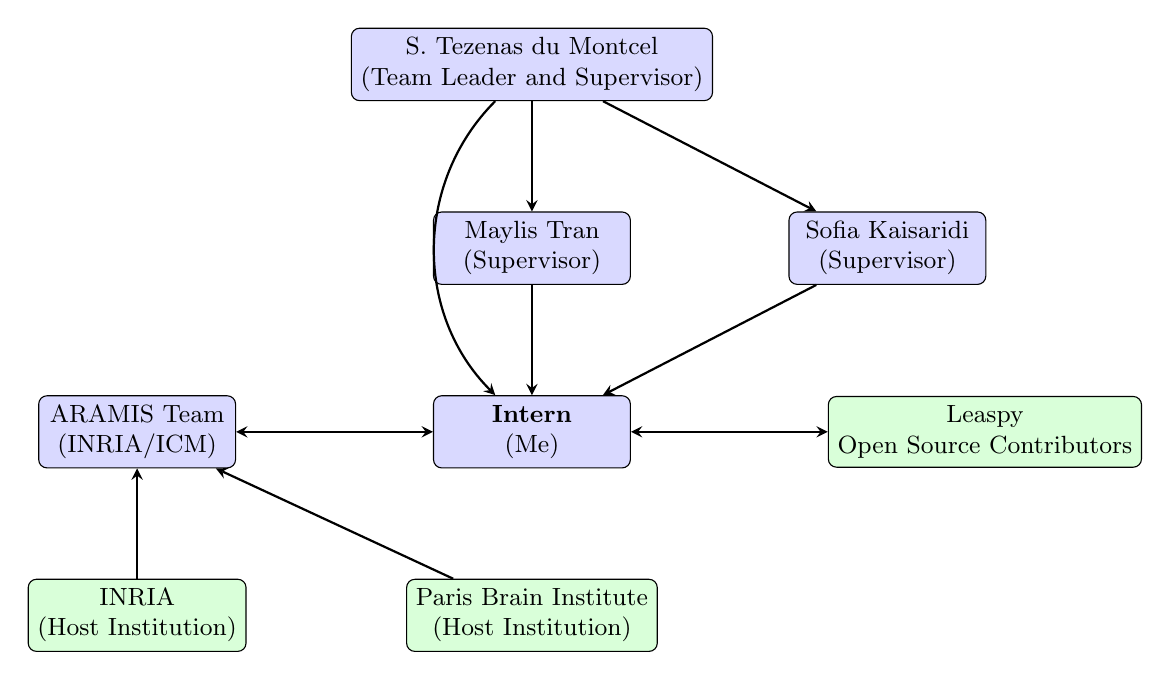
\begin{tikzpicture}[
    node distance=1.4cm and 2.0cm,
    box/.style={rectangle, rounded corners=3pt, draw, minimum width=2.5cm, minimum height=0.7cm, align=center, font=\small},
    intern/.style={box, fill=blue!15},
    extern/.style={box, fill=green!15},
    arrow/.style={->, >=stealth, thick}
]
 
\node[intern] (intern) {\textbf{Intern} \\ (Me)};
\node[intern, above=of intern] (maylis) {Maylis Tran\\(Supervisor)};
\node[intern, right=of maylis] (sofia) {Sofia Kaisaridi\\(Supervisor)};
\node[intern, above=of maylis] (sophie) {S. Tezenas du Montcel\\(Team Leader and Supervisor)};
\node[intern, left=of intern, xshift=-0.5cm] (aramis) {ARAMIS Team\\(INRIA/ICM)};
\node[extern, right=of intern, xshift=0.5cm] (leaspy) {Leaspy\\Open Source Contributors};
\node[extern, below=of aramis] (inria) {INRIA\\(Host Institution)};
\node[extern, below=of intern] (icm) {Paris Brain Institute\\(Host Institution)};
 
\draw[arrow] (maylis) -- (intern);
\draw[arrow] (sofia) -- (intern);
\draw[arrow] (sophie) -- (maylis);
\draw[arrow] (sophie) -- (sofia);
\draw[arrow] (sophie) to[bend right=45] (intern);
\draw[<->, >=stealth, thick] (intern) -- (aramis);
\draw[<->, >=stealth, thick] (intern) -- (leaspy);
\draw[arrow] (inria) -- (aramis);
\draw[arrow] (icm) -- (aramis);
\end{tikzpicture}
\caption{Network of internal and external actors involved in the internship.}
\label{fig:network}
\end{figure}

\section{Mission Reformulation and Context}

Neurodegenerative diseases such as Alzheimer's or Parkinson's disease progress over many years, manifesting through the simultaneous decline of motor abilities, cognitive scores, and physiological biomarkers. Understanding their trajectory is both a scientific challenge and a clinical necessity for early diagnosis and therapeutic evaluation.

Longitudinal clinical studies allow researchers to track biomarkers and clinical scores over multiple time points for a cohort of patients. These datasets also include critical patient events such as diagnosis date, surgical interventions, or death. Analyzing these heterogeneous, multivariate, and censored data jointly requires powerful statistical modeling.

Leaspy (LEArning Spatiotemporal Patterns in Python) was developed by the ARAMIS team to address this need. It is built on a nonlinear mixed-effects model (NLMEM) with a time reparameterization, enabling the estimation of both a population-level disease trajectory and individual patient parameters that capture inter-subject variability. Fixed effects are estimated via an iterative MCMC-SAEM algorithm, and individual random effects are estimated through various personalization methods. \\

\noindent The internship offer initially described two main tasks:

\begin{itemize}
    \item \textbf{Joint Model Simulation (Part 1):} Implement within Leaspy the ability to simulate patient events (e.g., time to diagnosis, death) jointly with longitudinal biomarker trajectories, using the joint spatiotemporal model. This requires both a theoretical understanding of the model and practical software development work.
 
    \item \textbf{Evaluation of Individual Parameter Estimation (Part 2):} Design and conduct a simulation study that benchmarks existing methods for estimating individual parameters (e.g., MAP, MCMC sampling). This involves proposing metrics for bias quantification and uncertainty estimation, and possibly implementing correction strategies.
\end{itemize}

\section{Strategic and Scientific Stakes}

From the team's perspective, this internship contributes to a core methodological objective: making Leaspy a more complete and statistically rigorous tool for the modeling of neurodegenerative disease progression. The improvements are relevant at multiple levels. Providing simulation tools for joint models enables the team to validate the statistical properties of their methods, which is essential before applying them to clinical datasets. The implementation work will also result in contributions to the Leaspy open-source library, which is used both internally and by external collaborators. Finally, accurate individual parameter estimation is a prerequisite for personalized patient prognosis, which is one of the long-term goals of the ARAMIS group.

\section{Work Plan and Preliminary Results}

\subsection{Macro Planning}

The internship spans approximately 6 months (April–September 2026). The main phases are outlined in Table~\ref{tab:planning}.

\begin{table}[h!]
\centering
\small
\begin{tabularx}{\textwidth}{|>{\raggedright\arraybackslash}X|>{\raggedright\arraybackslash}p{2.2cm}|>{\raggedright\arraybackslash}X|}
\hline
\textbf{Phase} & \textbf{Period} & \textbf{Key Activities / Decision Points} \\
\hline
Onboarding \& Literature Review & April & Read core references; understand Leaspy codebase; set up development environment \\
\hline
Part 1: Joint Model Simulation & April - May & Implement event simulation; unit tests; \textbf{Milestone: first working simulation} \\
\hline
Part 1: Validation \& Integration & May - June & Validate outputs; integrate into Leaspy; code review with supervisors \\
\hline
Part 2: Simulation Study Design & June & Define metrics; identify scenarios; \textbf{Milestone: study protocol validated by supervisors} \\
\hline
Part 2: Execution \& Analysis & June - August & Run experiments; statistical analysis; compare methods \\
\hline
Report Writing \& Presentation & August - September & Write internship report; prepare final presentation; \textbf{Defense} \\
\hline
\end{tabularx}
\caption{Macro planning of the internship, with key milestones and decision points.}
\label{tab:planning}
\end{table}

\subsection{Feedback and Evaluation Process}

Regular meetings with both supervisors (Maylis Tran and Sofia Kaisaridi) are held weekly, allowing for continuous feedback on both the scientific content and the software development progress. Major milestones (completion of Part 1, study protocol for Part 2) will be reviewed collectively with the team leader. This first progress report marks a formal evaluation checkpoint, and a final internship report and oral defense will conclude the evaluation process.

\subsection{Preliminary Results: Joint Model Simulation}

At this stage of the internship, the work has focused on Part 1. After familiarizing myself with the Leaspy codebase and the joint model formulation, I have begun implementing simulation functions for patient events.

The following figures present preliminary results of the joint model simulation. They illustrate simulated longitudinal biomarker distributions and event times for a synthetic cohort of patients on a toy dataset. 

\begin{figure}[h!]
\centering
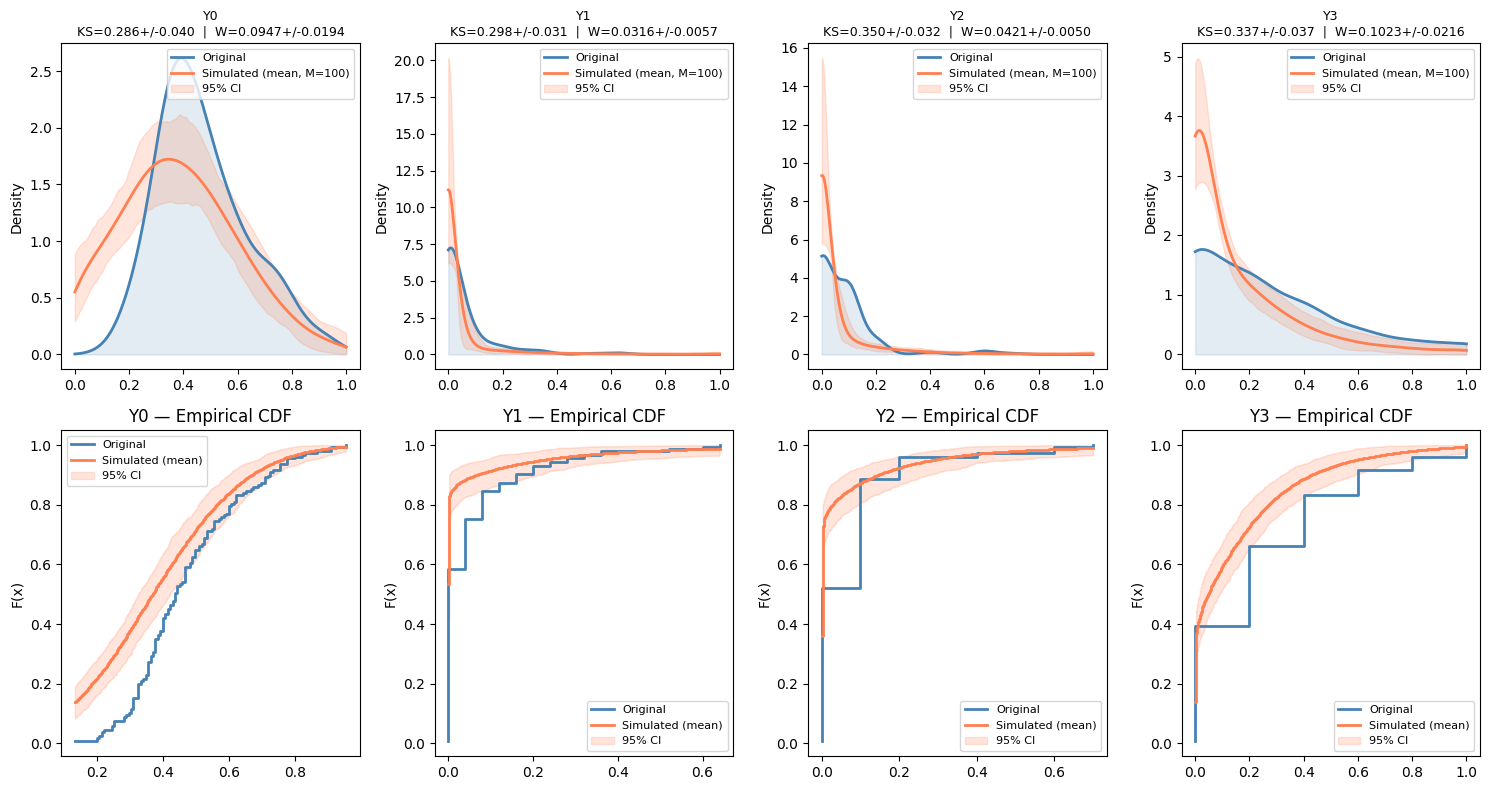
\includegraphics[width=0.8\textwidth]{figures/prelim_distrib.png}
\caption{Comparison of original (blue) and simulated (orange) biomarker density distributions and CDFsusing the joint model on a toy dataset available in Leaspy.}
\label{fig:prelim_distrib}
\end{figure}

\begin{figure}[h!]
\centering
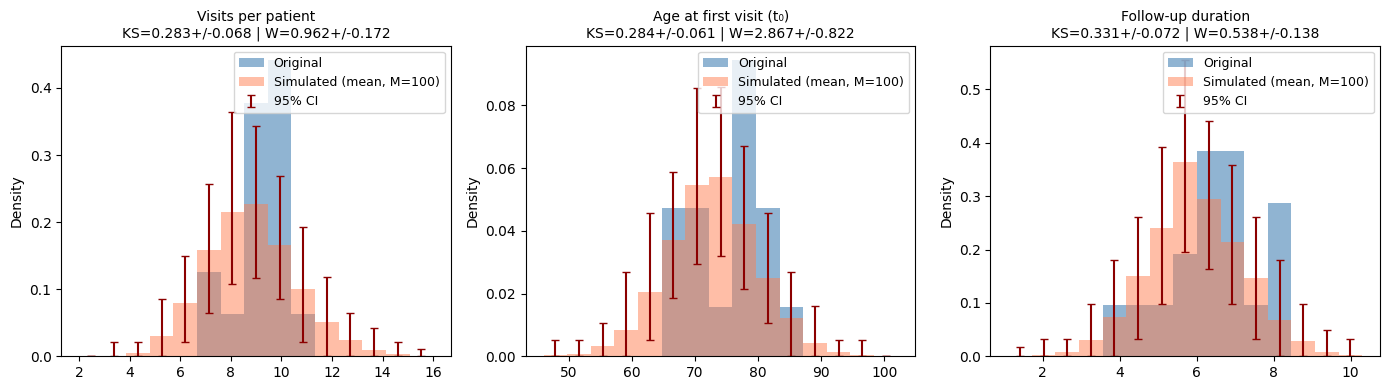
\includegraphics[width=0.8\textwidth]{figures/prelim_events.png}
\caption{Comparison of original (blue) and simulated (orange) event time distributions using the joint model on a toy dataset available in Leaspy.}
\label{fig:prelim_events}
\end{figure}

\end{document}
